\subsection{Gameplay}

\subsubsection{Système de verrouillage}

Pour tuer un personnage (joueur ou NPC),
nous avons ajouté un système de verrouillage. Celui-ci est assez pratique, lorsque l'on passe dans ce mode, l'écran change,
un effet réalisé grâce au post processing de Unity permet de donner un effet sépia/vieux films\footnote{voir Effets Graphiques}.
Un contour blanc autour des personnages visés au centre de l'écran permettent voir quel personnage va être sélectionné.

Une fois sélectionné et lorsque le joueur est proche de sa cible, il peut alors l'éliminer.

L'effet a demandé de créer plusieurs overlay de caméra, afin d'avoir un effet graphique
appliqué uniquement sur certains layers, et de les surperposer les unes sur les autres. 

\subsubsection{Finishers}
Nous avons fourni un vrai travail sur les différentes animations de morts des personnages.
Lors de sa réalisation, un problème s'est posé : Il fallait que les animations de deux GameObject (ici le joueur qui tue et le NPC/joueur tué) 
soient synchronisées et très précises spatialement. Après avoir regardé plusieurs types de solutions, nous nous sommes tournés vers un outil préintégré nommé Timeline.
Ce dernier permet de réaliser des clips vidéos.

Voici donc comment nous avons intégré les timelines :
\newline
Des faux personnages jouant les animations sont ajoutés sur la cartes à la position et rotation du tueur.
On masque le tueur et le tué de la carte.
On change le mesh et le matériau de chaque personnage de la timeline pour qu'il corresponde au tueur et au
personnage tué.

Une fois l'animation terminé, un signal est envoyé à script qui réaffiche alors le joueur qui était masqué.
Si la personnage tué était un joueur, alors il réapparait discrètement ailleurs sur la map lors de sa réaparition.
Le personnage tué disparait de la carte au bout d'une dizaine de secondes avec un shader fait avec Shader Graph.

Voici quelques finishers que nous avons réalisé :

\begin{figure}[hbt!]
    \centering
    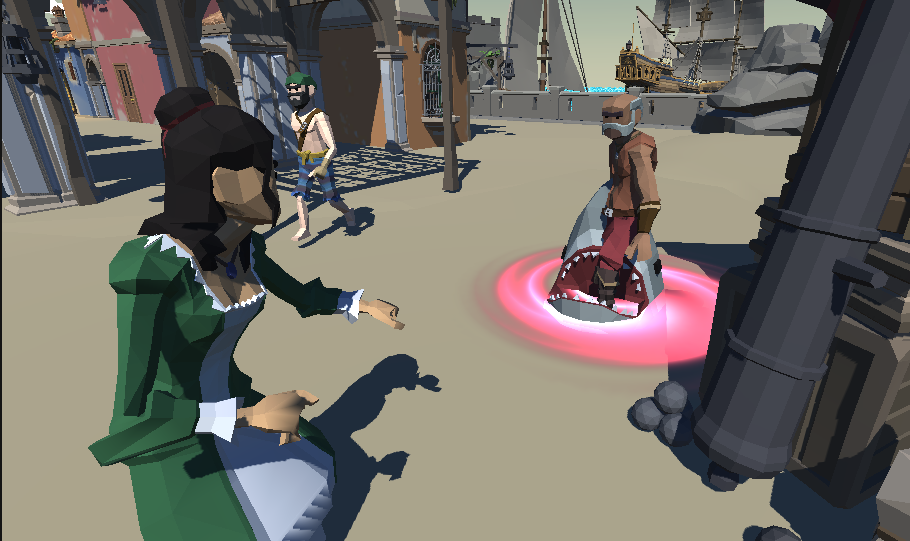
\includegraphics[scale=0.3]{finishers/shark.png}
	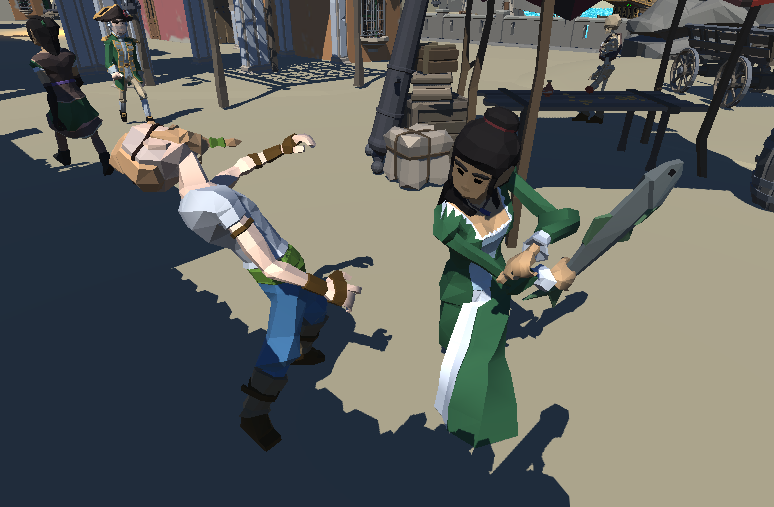
\includegraphics[scale=0.3]{finishers/fish.png}
	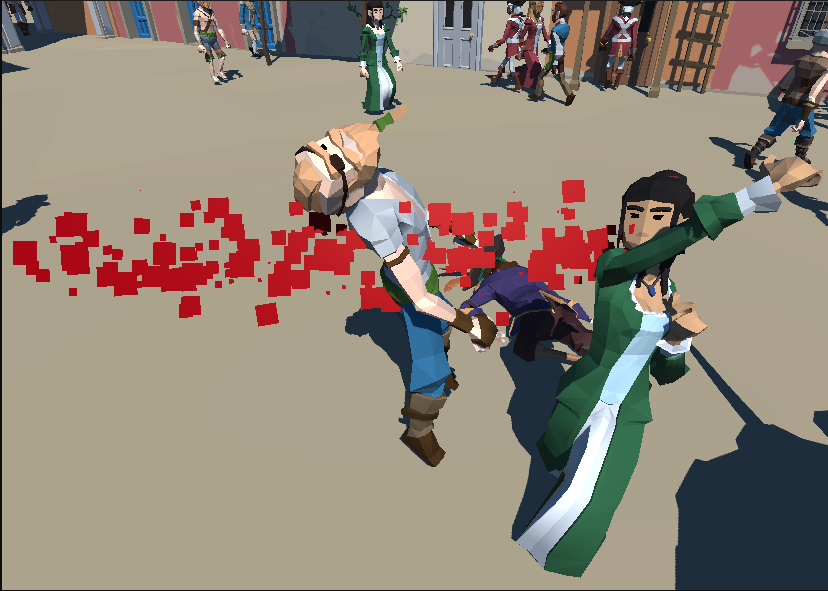
\includegraphics[scale=0.3]{finishers/hand.png}
	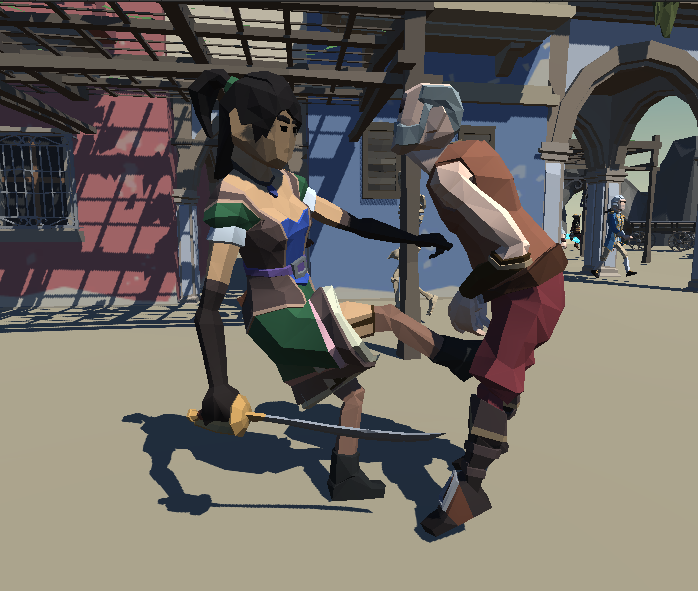
\includegraphics[scale=0.3]{finishers/balls.png}
    \caption{Quelques finishers}
\end{figure}
\FloatBarrier


\subsubsection{Système de manche}
    Le système actuellement utilisé pour le déroulement d'une partie se base sur des manches. Le jeu se fait en deux phase:
    	-Une période de 'grâce' de 30 secondes où les joueurs attendent l'assignation d'une cible. 
	 Ils sont libre de se déplacer, pour se cacher par exemple.

	-Une période de 'chasse'. Les cibles sont assignés et le combat peut commencer. Elle est au départ de 3 minutes, mais ce temps
	 diminue à chaque mort de joueur pour pousser les participants au meurtre.

\subsubsection{Système de mort}
    Joueurs comme IA peuvent être tués. Dans le cas d'un joueur, un système de mort a été mis en place. Ainsi,
    quand le joueur se fait tuer, son personnage est désactivé temporairement et il rentre
    en mode "spectateur". Il peut se balader sur la map, mais il ne peut en aucun cas interagir avec l'environnement,
	et il n'est pas visible des autres joueurs.

\subsubsection{Système de point}
    Un système de point a également été implémenté. Il fonctionne de la façon suivante:
    
	-Tuer sa cible rapporte des points. le premier joueur tuant sa cible gagne plus de point, les autres en gagne de moins en moins.
	
	-Tuer une IA fait perdre des point! Il faut donc faire attention à ne pas tuer n'importe qui. Celà encourage la réflexion et pas 	 simplement un carnage afin de trouver sa cible.
	
	-Tuer la cible de quelqu'un d'autre ne fais pas perdre de points, mais un système de compensation a été mis en place. Ainsi, se 	faire voler sa cible par un autre joueur apporte des points de compensation. Encore une fois, il n'est donc pas dans l'intérêt 
	des joueurs de tuer le premier venu!

	-Une autre façon de gagner des points et d'être encore en vie à la fin d'une manche.

    Bien évidemment, tout cela est dans le but de déterminer le vainqueur.
